\documentclass{article}
\usepackage[utf8]{inputenc}
\usepackage{graphicx}

\title{Tarea 1}
\author{Sanchez Leyva Eduardo Samuel}
\date{\today}

\begin{document}

\maketitle

\newpage

\section{Biografía de John Guttag}
\textbf{¿Quién es John Guttag?}
\\

\par

John Vogel Guttag es un científico informático estadounidense, anteriormente fue profesor del MIT, a cargo de enseñar Ingeniería Eléctrica y Ciencias de la Computación.Nacio el 6 de  Marzo de 1949, de nacionalidad Estadounidense, actualmente con 73 años de edad, experto en las ciencias de la computación. \\

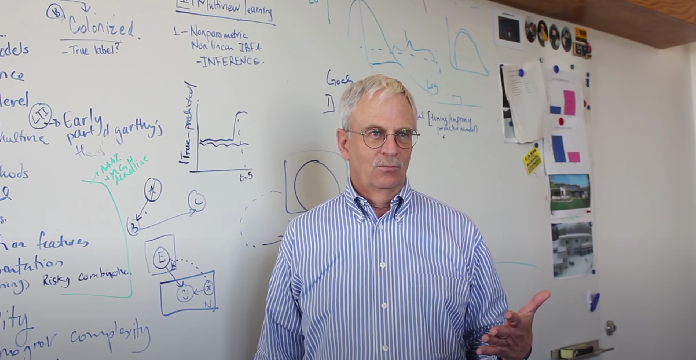
\includegraphics[scale=0.55]{image.png}

\textbf{Educación y enseñanza}

En la Universidad de Brown, el año de 1971 se recibió, recibiendo un titulo de licenciatura en ingles, y para el año posterior, recibir una maestria en matemáticas aplicadas de Brown.\\
\par En la Universidad de Toronto, el año de 1975 recibio un doctorado en Ciencias de la Computación.
Miembro de la facultad de la Universidad del Sur de California entre los años 75 a 78. Posteriormente, en 1979 se unió a la enseñanza en el Instituto de Tecnologia en Massachusetts, más conocido como MIT(Massachusetts Institute of Technology), una universidad privada en Cambridge, Estados Unidos, y considerada de las más prestigiosas universidades a nivel mundial.

\textbf{Aportes a MIT}
Se ha desempeñado como Jefe asociado del departamento Ingenieria Electrica y Ciencias de la Computación. Tamien como jefe de departamento, sus aportes a la facultad son bastantes. Uno de los fundadores de Health Scale Technologies, empresa de aprendizaje automatico e inteligencia Artificial.\\ 
\par En los ultimos años, el se encuentra ayudando estudiantes a aprender y aplicar modos computacionales de pensamiento para enmarcar problemas y guiar el proceso de extracción útil para datos.\\
\par Tiene libros de temas de computación y programación, y cuenta con diversos cursos MIT OpenCourseWare, entre ellos la introducción a la programación y Ciencias de la Computación, Data Science, Computational Thinking, etc.\\

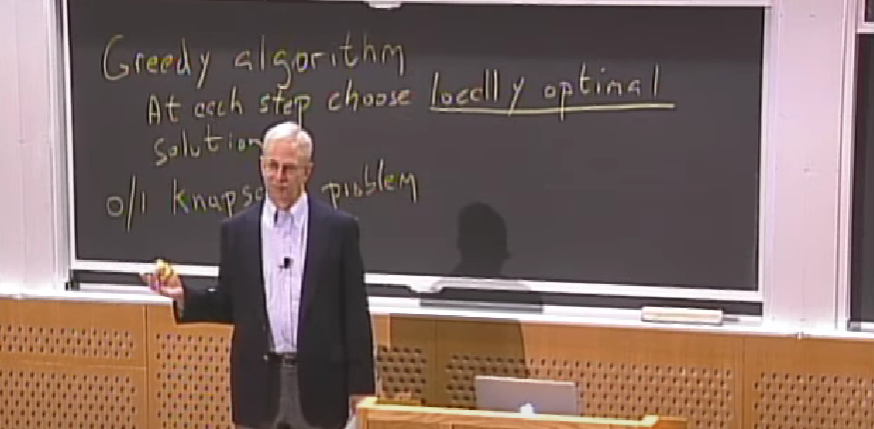
\includegraphics[scale=0.45]{image2.png}

\par Dirige el Grupo de Máquinas Clínicas y Aplicadas del Laboratorio de Ciencias de la Computación e Inteligencia Artificial del MIT. El grupo desarrolla y aplica técnicas avanzadas de aprendizaje automático y visión por computadora a una variedad de problemas clínicamente relevantes. Los proyectos de investigación actuales incluyen la predicción y reducción de eventos médicos adversos, la coincidencia de pacientes con terapias y proveedores, y las imágenes médicas.\\
\par Ha publicado esta investigación en lugares de aprendizaje automático, inteligencia artificial general y visión por computadora, así como en conferencias y revistas de orientación médica.

\section{Biografia de Barba Liskov}


\end{document}
